%\documentclass[a4paper]{article}
\documentclass[journal]{IEEEtran}

\usepackage[pdftex,pdfauthor={Shabaz Sultan, Chi Chun Wan, Boudewijn Zwaal},pdftitle={Airline sc},colorlinks=true, linkcolor=black,          % color of internal links
    citecolor=black,        % color of links to bibliography
    filecolor=black,      % color of file links
    urlcolor=black   ]{hyperref}
\usepackage[pdftex]{graphicx}
\usepackage{amsmath}
\usepackage{float}

\author{Chi Chun Wan -- 2525244\\
Shabaz Sultan -- 2566703\\
Boudewijn Zwaal -- 1897527}
\title{Airline Scheduling with Simulated Annealing}
\begin{document}
\maketitle



\begin{abstract}
%\boldmath
Abstract text to go here.
\end{abstract}


\section{Introduction}
Flight schedules take up a central place in airline businesses. To maximize profit a business has to be as efficient as possible in using its resources and be as effective as possible in meeting marketplace demand. A business wants to plan its flights based on demand, use its airplanes to service these flights as efficiently as possible and assign crews to these flights to minimize expenses. These pose highly complex combinatorial optimization problems that cannot be solved analytically. Instead numerical optimization systems are used and their effectiveness can be influential on the profitability of a passenger focusses airline as a whole.\\
The Dutch airline KLM flies on 150 destinations with 97 airplanes and needs to produce a flight schedule four times a year that maximizes their profitability \cite{Bian2003}. In this paper we will consider this problem in a slightly reduced scenario, with a fictional Mokum Airways that flies on 28 destinations with 6 airplanes. The goal is to maximize profit as measured by revenue passenger kilometers, often used as unit to measure the product being sold in a passenger focussed airline \cite{Schefczyk1993}. In order to obtain the best flight schedule, we use heuristics algorithms to analyze all the possible tours and find the optimal one.\\

\section{Background}
Constructing airline schedules can be broken down in a number of subproblems, each posing a number of computational and algorithmic challenges. Often first the flights that are provided by an airline are constructed, usually subject to complex regulation and non-deterministic customer demand functions. This is referred to as the Airline Scheduling problem in the literature, where the goal is to maximize profits by meeting said demands \cite{Etschmaier1985}. \\
The next step is to assign the flights that are flown to airplanes. This is the so-called Fleet Scheduling Problem \cite{Rushmeier1997}. An airplane schedule can be constructed ahead of time, but scheduling methods for real world scenarios need to deal with real-time adjustments as well due to delays on the day itself (e.g. due to weather conditions, technical problems or issues at an airport). Ideally these schedules are repeatable (usually over either a one or seven day period), requiring that if at the start of the day an aircraft is at airport A, there needs to be an aircraft (not necessarily the exact same, just one of the same type) at airport A at the end of the schedule. \\
Finally crew personnel is assigned to the flights and airplanes. The crew scheduling problem is subject to constraints from flight authority regulation, labour regulation and airline specific regulation and because it represents the largest expenditure for airlines after fuel cost it is an important area of research for the industry as well \cite{Gopalakrishnan2005}.\\
This paper tackles the design and optimization of an airline schedule, with airplane assignment being part of the designed schedule. The one consideration given to the constraints from the crew schedule problem is that the schedule needs to have single homebase, each crew member is assumed to live at said homebase and each plane needs to attend that homebase daily for a crew change.\\
There are various approaches to this problem, such as integer programming \cite{Raff1983} or even agent based approaches \cite{Langerman1997}. One candidate for complex combinatorial optimization problems in general is Simulated Annealing \cite{kirkpatrick1983optimization}. This meta-heuristic has been applied to related problems such as crew scheduling \cite{Sosnowska2001}. It has been specifically used for airline scheduling by \cite{Mashford2001}, which is the main reference for the research described in this paper.
\section{Problem}
There are multiple formalisations of the problem to be found in the literature. We mostly follow \cite{Mashford2001}, because it most closely matches our research. Let $X$ be the set of nodes representing the airports. $G \subset X \times X$ is the service graph, making up all the valid flightpaths between two airports. In the example scenario we consider this will be the full Cartesian product between all airports, see figure~\ref{fig:service_graph}.
\\
\begin{figure}[!h]
\centering
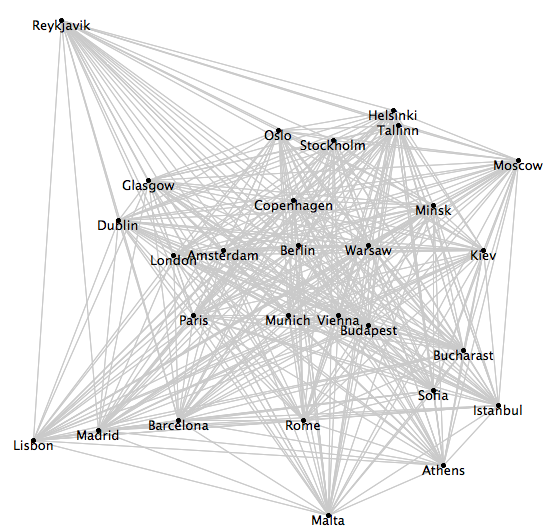
\includegraphics[width=2.3in]{service_graph}
\caption{Service graph.}
\label{fig:service_graph}
\end{figure}
\\
We schedule over an interval $[T_1, T_2]$, with $T_1 < T_2$. The fleet is defined as $F = \{p_1 \cdots p_n\}$, with $p_i$ being an airplane. The schedule for a plane is a list of flights, which are defined as quadruples $(x, y, t, p)$, with $x \in X$ the flight origin, $y \in X$ the destination, $t \in [T_1, T_2]$ the departure time and $p\in F$ the plane. \\
An airline schedule is then defined as [TODO]
\section{Algorithm}
To deal with the problem, we use two heuristic algorithms, namely hill-climbing and simulated annealing for six airplanes and one algorithm brute force for one airplane.

\subsection{Brute-force}
Brute-force is a problem-solving technique that consists of systematically enumerating all possible candidates for the solution and checking whether each candidate satisfies the problem's statement. In our case, we check all the possible tours by using a tree structure, where the node represents the destinations. A representation of the tree is given in figure~\ref{fig:tree}.\\
\begin{figure}[!h]
\centering
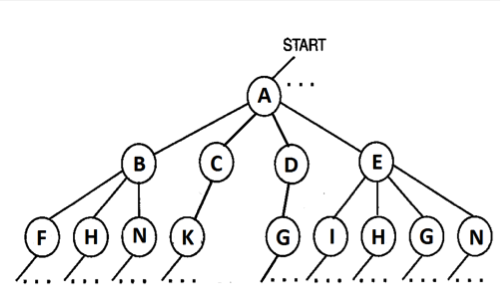
\includegraphics[width=2.5in]{tree}
\caption{Tree data structure}
\label{fig:tree}
\end{figure}
\\
An advantage of this algorithm is that the solution found, also is  the optimal solution. A disadvantage is that the run time will increases a lot to find a solution, when the state space is big. Therefore, we add branch and bound to the algorithm. The branch and bound algorithm has a upper-and lower bound. The upper bound is the theoretical maximum passengers-kilometer score and the lower bound is the best founded score so far for every step. For every position in the tree, we calculate what the maximum score is that can still be obtained from that position. If the score is lower than the current lower bound. We will not look further anymore from that position. This has as result that it will make the possibilities smaller and therefore a lower run time. 
\subsection{Hill-climbing}
Hill-climbing is an iterative algorithm that starts with an arbitrary solution to a problem, then attempts to find a better solution by changing a single element of the solution. If the change produces a better solution, an incremental change is made to the new solution, repeating until no further improvements can be found.\\
In the case of our problem, a flowchart is made in figure~\ref{fig:flowchart_hc}.\\
\begin{figure}[!h]
\centering
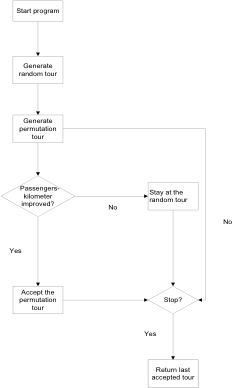
\includegraphics[width=2.5in]{flowchart_hc}
\caption{Flowchart Hill-climbing}
\label{fig:flowchart_hc}
\end{figure}
\\
We start with an initial random tour. To find a better solution, we permutate the tour by randomly selecting a sub-tour in the initial tour and replace it with another possible valid sub-tour. Care is taken to not remove the home-base airport from the tour. The score of the passenger-kilometers for the initial tour is stored in a variable best score. If the score of the permutation tour is higher than the score of the arbitrary tour, the score of the permutated tour will be the new best score and the permutation tour will be accepted, otherwise the best score will stay the same and we will stay at the previous tour. This process is repeated until no further improvements can be found and the best tour is the last accepted tour. When applied to multiple planes, first one of the planes in the system is randomly chosen and its flightplan (tour) is permutated. The total score of all airplane tours is then calculated and compared to the previous best score. If it improves on said score, the new tour is accepted.\\
A disadvantage of hill-climbing is that it is good for finding a local optimum, but it is not guaranteed to find the best possible solution (global optimum). To avoid this disadvantage, we use a different algorithm, simulated annealing. \\
\subsection{Simulated Annealing}
In case of simulated annealing, it’s almost the same as hill climbing except when the solution is not improved, this solution will be accepted with a probability P. The probability is based on the number of iterations and the temperature. As the number of iterations increases, the temperature goes down and the probability will decrease. \\
In figure~\ref{fig:flowchart_sa}, the flowchart of hill-climbing is adjusted in simulated annealing.\\
\begin{figure}[!h]
\centering
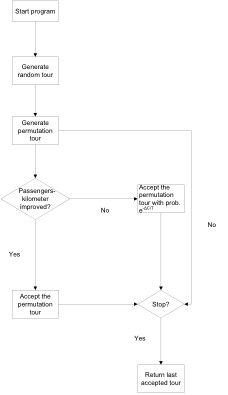
\includegraphics{flowchart_sa}
\caption{Flowchart Simulated Annealing}
\label{fig:flowchart_sa}
\end{figure}
\\
In the case when the passengers-kilometer score is not improved, you will accept the permutation tour with probability $P = e^{\frac{−\Delta C}{T}} $, where ∆C = score of the permutation tour − score of the current best tour and $T = 0, 999^i * T_0$ with $i$ is the number of iterations and $T_0$ is the start temperature 50.000.
 This probability will decrease with the number of iterations. Thus when the number of iterations increases, the temperature goes down. When temperature is high, the system will choose new states more or less at random, but as the temperature lowers this algorithm will go to hill-climbing. 
\section{Result}
To validate our method, demand and flight distances for a fictional airline are used. Mokum Airways, a newly created Dutch airline based in Amsterdam, has landing rights for 28 destinations around Europe.\\
\begin{figure}[!h]
\centering
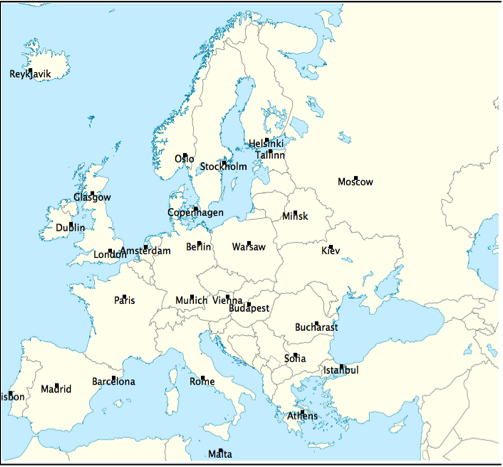
\includegraphics[width=2.5in]{europe}
\caption{Mokum Airways destinations}
\label{fig:europe}
\end{figure}
\\
The airline has a fleet of six Airbus A321 aircrafts with speed of 800km/h, capacity of 199 and range of 3199 km.  The take-off and landing take place between 02:00 and 06:00 and docking time and refuel time will take one hour. Moreover, once per day the plane needs to land in the home-base for the crew-change. The flight schedule has to be a cycle, so the start point and the end point of the route has to be the same. \\
\begin{figure}[!h]
\centering
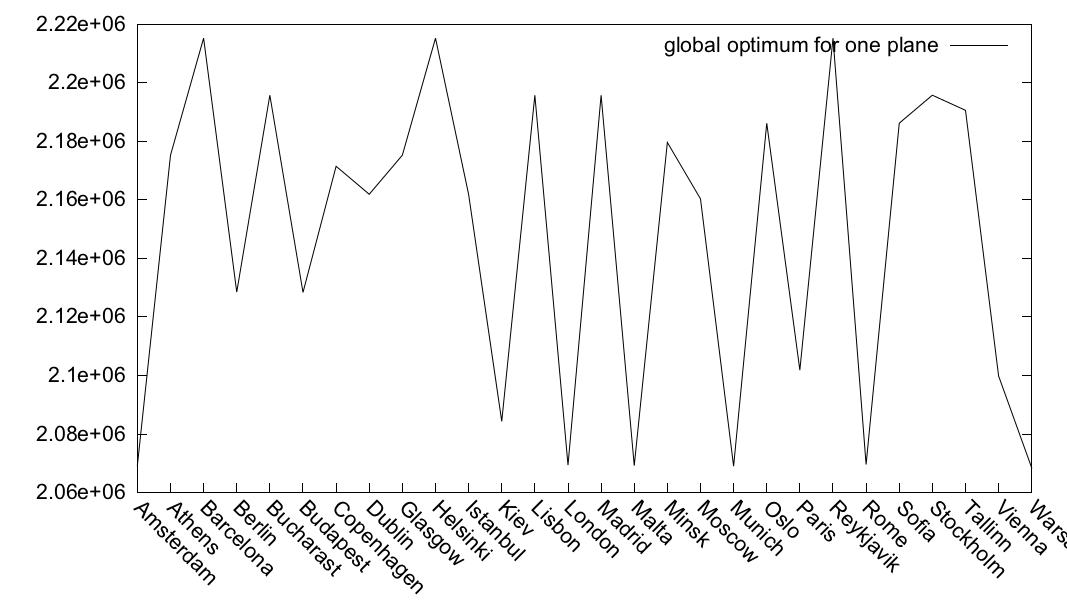
\includegraphics[width=2.5in]{different_homebases_one_plane}
\caption{Global optimum for different homebases with one plane}
\label{fig:different_homebase_one_plane}
\end{figure}
\\
\begin{figure}[!h]
\centering
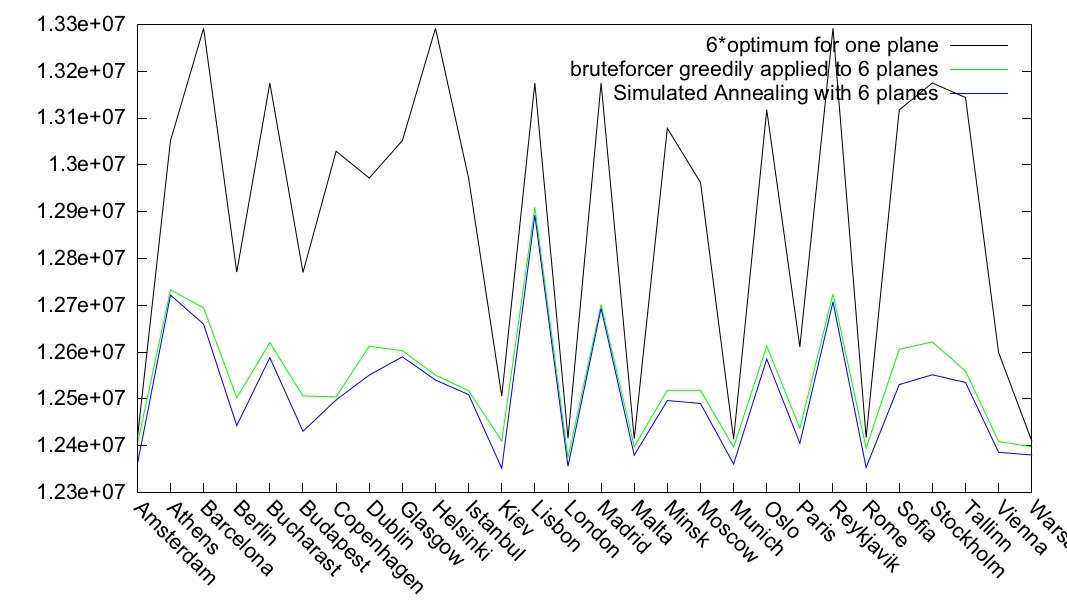
\includegraphics[width=2.5in]{different_homebases}
\caption{Results for different homebases with six planes, Simulated Annealing line based on best of 5 runs for each scenario, cooling rate of $0.99999$.}
\label{fig:different_homebase_six_planes}
\end{figure}
\\
\begin{figure}[!h]
\centering
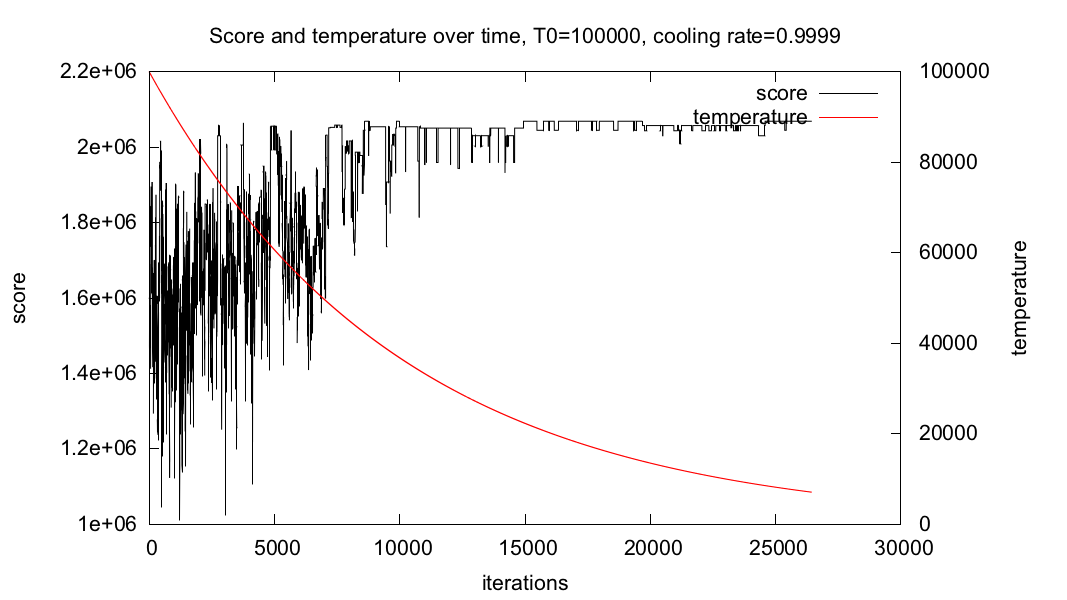
\includegraphics[width=2.5in]{score_over_time}
\caption{Score over time for Simulated Annealing}
\label{fig:simulated_annealing_score}
\end{figure}
\\
\begin{figure}[!h]
\centering
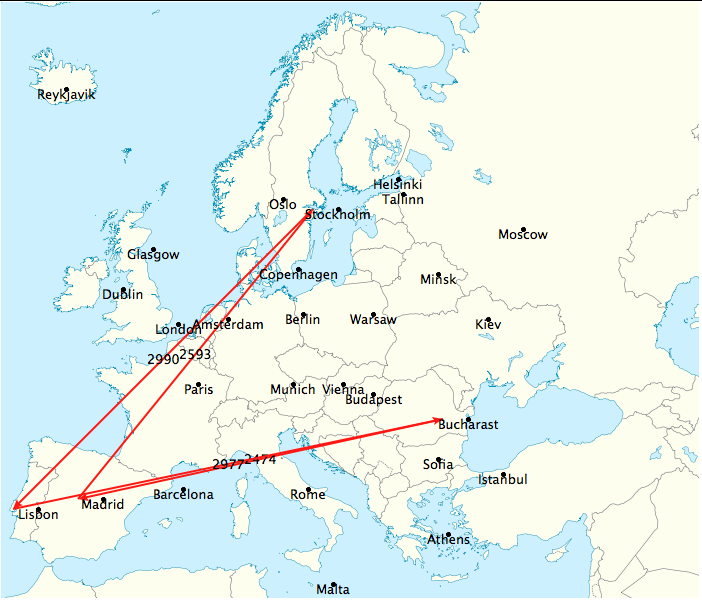
\includegraphics[width=2.5in, trim=0 0 0 2, clip=true]{best_tour_one_plane}
\caption{Best tour for one plane with homebase Amsterdam, passenger kilometer score 2069202.}
\label{fig:one_plane_amsterdam}
\end{figure}
\\
\begin{figure}[!h]
\centering
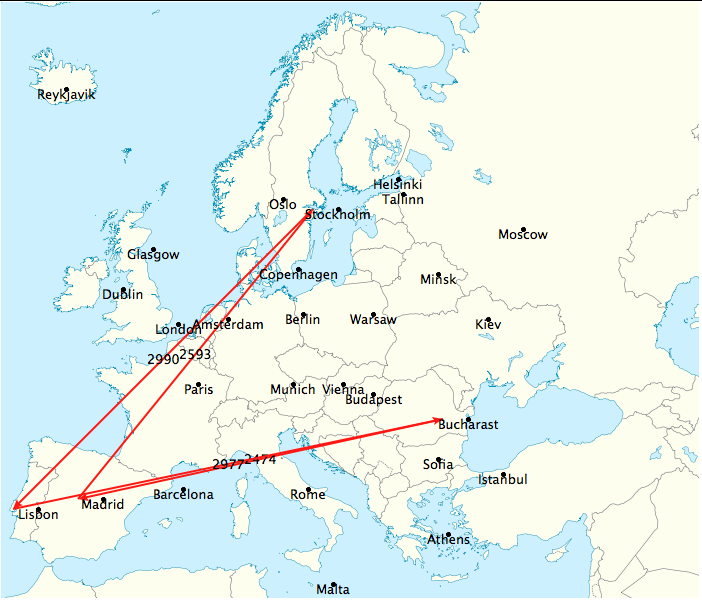
\includegraphics[width=2.5in, trim=0 0 0 2, clip=true]{best_tour_one_plane}
\caption{Best tour for one plane with any homebase, passenger kilometer score 2195766.}
\label{fig:one_plane}
\end{figure}
\section{Analysis}
To analyze the quality of the heuristic algorithms, Hill-climbing and simulated annealing. We use the result of the brute force for one airplane as reference, since the result is the global maximum. In graph 1, the RMSE of the score for simulated annealing is plotted. When the iterations increase, the RMSE will decrease. The number of iterations depends on the cooling rate, a lower cooling rate will 
\begin{figure}[!h]
\centering
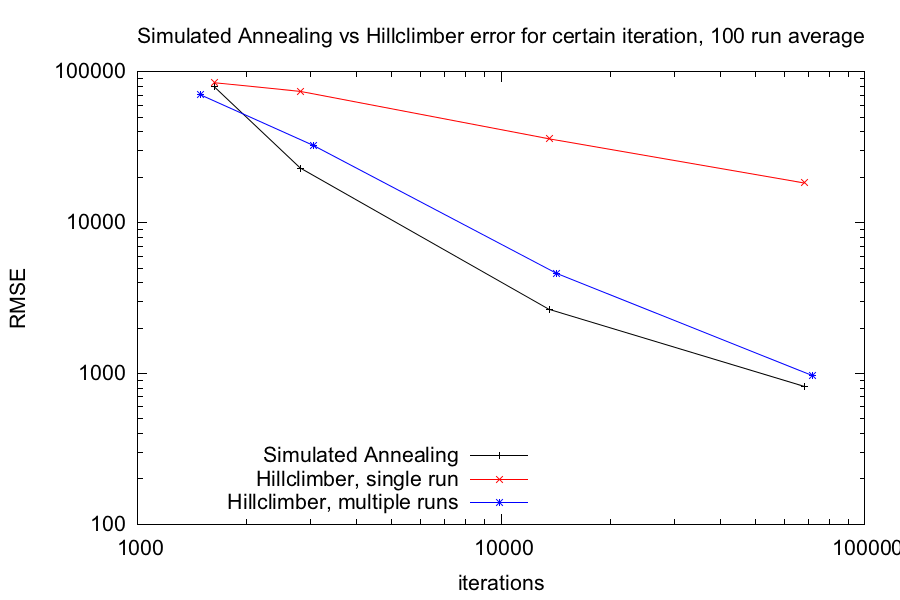
\includegraphics[width=2.5in]{iterations_vs_error_sa_hc}
\caption{Error for Simulated Annealing and Hill-climbing.}
\label{fig:error_sa_hc}
\end{figure}
\section{Conclusions}
\bibliographystyle{IEEEtran}
\bibliography{final_report}
\end{document}

